\section{Evaluation}\label{sec:eval}

We evaluate \( \tool \) based on the following four research questions:
\begin{itemize}
  \item RQ2) \textbf{Effectiveness} Is \( \tool \) effective to extract syntax and
    semantics of existing ECMAScript specifications?
  \item RQ1) \textbf{Correctness} Does \( \tool \) correctly extract JavaScript syntax
    and semantics from ECMAScript 2020 speicification?
  \item RQ3) \textbf{Adaptability} Does \( \tool \) deal with future proposed features?
  \item RQ4) \textbf{Specification Error Detection} What specification errors
    are detected by \( \tool \)?
\end{itemize}

\subsection{Effectiveness}

\begin{figure}[t]
  \centering
  \begin{subfigure}{0.48\textwidth}
    \[
      \begin{array}{c|r|r|r|r|r}
        \hline
        \text{version}
        & \multicolumn{1}{c|}{2016}
        & \multicolumn{1}{c|}{2017}
        & \multicolumn{1}{c|}{2018}
        & \multicolumn{1}{c|}{2019}
        & \multicolumn{1}{c}{2020}\\\hline
        \text{\#prods}
        & \text{\inred{XXX}}
        & \text{\inred{XXX}}
        & \text{\inred{XXX}}
        & \text{\inred{XXX}}
        & \text{\inred{XXX}}\\\hline
        \Delta
        & \multicolumn{1}{c|}{\text{-}}
        & \text{\inred{XXX}}
        & \text{\inred{XXX}}
        & \text{\inred{XXX}}
        & \text{\inred{XXX}}\\\hline
      \end{array}
    \]
    \caption{The parser generator.}
    \label{fig:syntax-all-version}
  \end{subfigure}
  \begin{subfigure}{0.48\textwidth}
    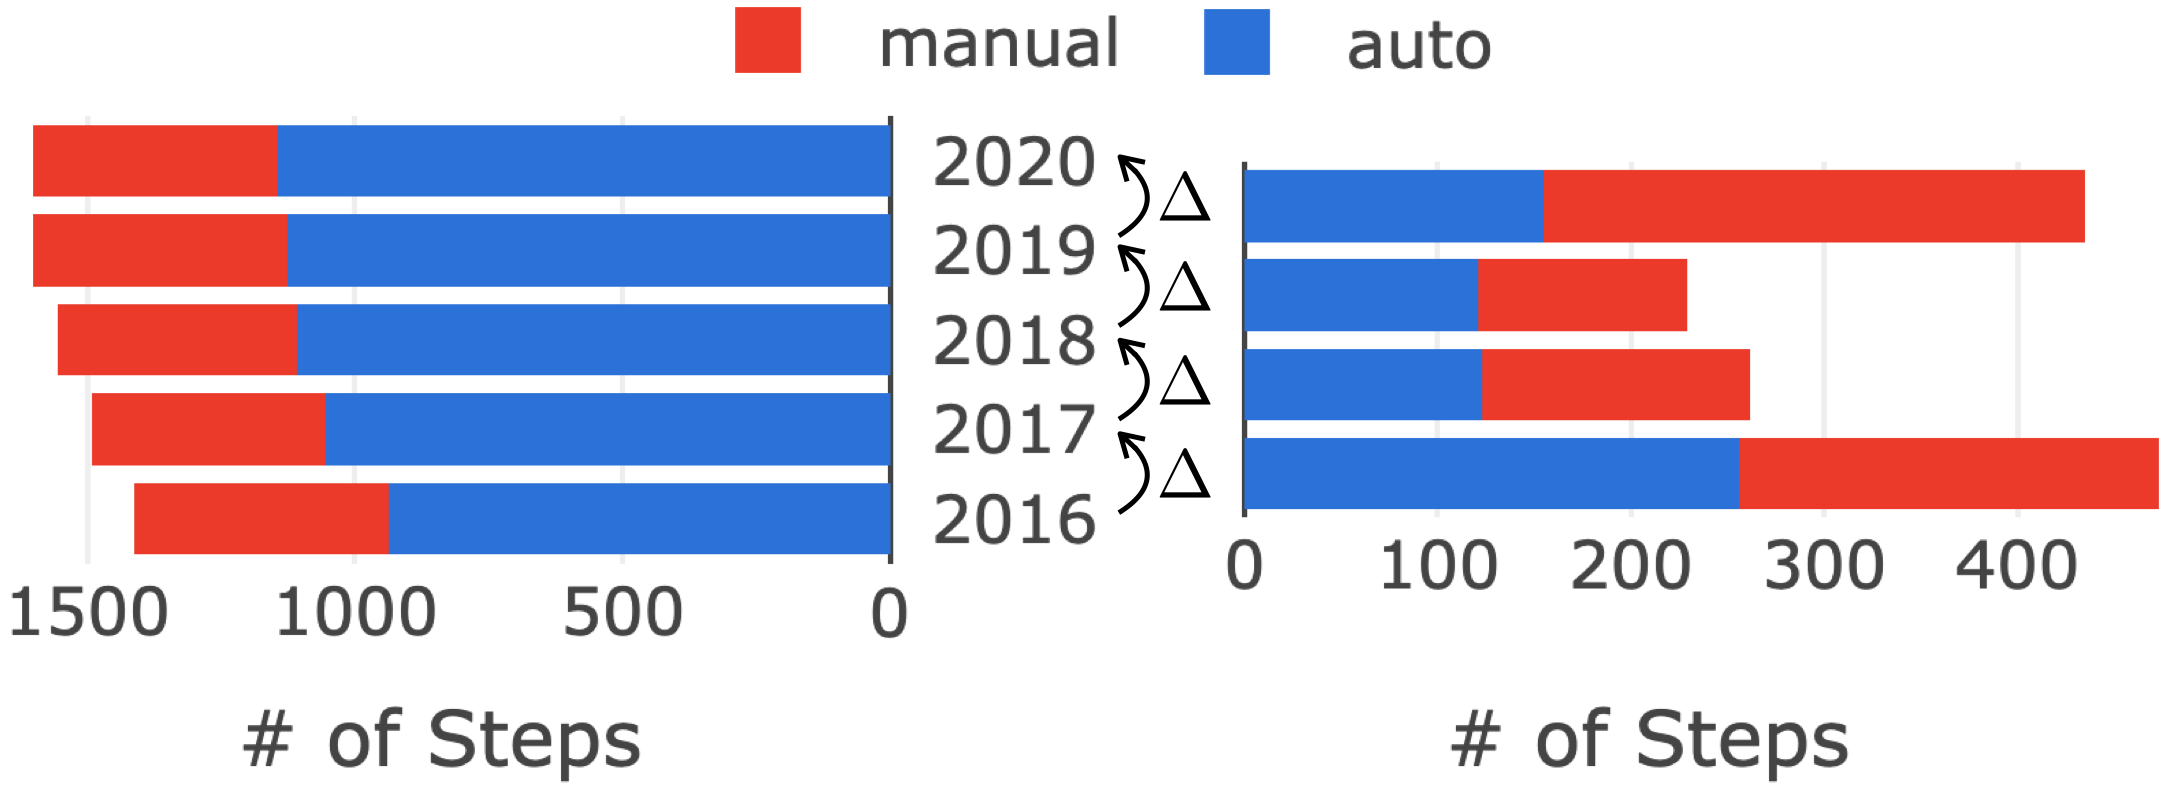
\includegraphics[width=\textwidth]{img/all-version-sem.png}
    \caption{The algorithm compiler.}
    \label{fig:semantics-all-version}
  \end{subfigure}
  \caption{The result of the parser generator and the algorithm compiler for
  ECMAScript specifications from 2016 to 2020.}
  \label{fig:all-version}
\end{figure}

We discuss the effectiveness of \( \tool \) by applying it into existing ECMAScript specifications.
The evaluation focuses on how many productions and abstract algorithms are covered by
our tool 1) in each version, and 2) in each difference between adjacent versions.
Figure~\ref{fig:all-version} shows the result of \( \tool \) from ECMAScript 2016
to 2020. While ECMAScript 5.1 is the first version that officially supports
the specification in HTML. However, two oldest versions ECMAScript 5.1 and 2015 are written
in quite different styles with recent versions including HTML tags used in abstract algorithms.
Thus, we evaluate only five recent versions from ECMAScript 2016 to 2020.
As described in Figure~\ref{fig:all-version}, \( \tool \) suceeds to generate parsers
from all versions. For semantics, the algorithm compiler has \inred{XX\%} success rates
in average. Moreover, \( \tool \) are also effective to update existing semantics
because \inred{XX\%} of newly defined algorithms are automatically compiled into \( \ires \)
functions.

\subsection{Correctness}

\begin{table}
  \centering
  \begin{tabular}{lr}\toprule
    \belowrulesepcolor{gainsboro}
    \rowcolor{gainsboro} \textbf{All tests262 Tests} & \textbf{36,794} \\
    \aboverulesepcolor{gainsboro}\midrule
    Annexes/Internationalisation & 1,774\\ \hdashline
    In-progress features & \inred{XXXX} \\\hdashline
    Module tests & \inred{XXXX} \\\hdashline
    Non-strict tests & \inred{XXXX} \\\midrule
    \belowrulesepcolor{gainsboro}
    \rowcolor{gainsboro} \textbf{ECMAScript 2020 Strict Script Tests} & \textbf{\inred{XXXXX}} \\
    \aboverulesepcolor{gainsboro}\midrule
    Not supported features & \inred{XXXX} \\\midrule
    \belowrulesepcolor{gainsboro}
    \rowcolor{gainsboro} \textbf{Applicable Tests} & \textbf{\inred{XXXXX}} \\
    \aboverulesepcolor{gainsboro}\midrule
    Passed tests & \inred{XXXX} \\\hdashline
    Failed tests & \inred{XXXX} \\\bottomrule
  \end{tabular}
  \caption{The results of tests in the test262 for ECMAScript 2020.}
  \label{table:test262}
\end{table}

To evaluate that \( \tool \) correctly extracts semantics, we extract semantics of ECMAScript
2020 via our tool. Above automatically extracted parts of semantics, we manually implement
\inred{XX} \( \ires \) functions for abstract algorithms failed to be automatically compiled.
Moreover, we fill in global setting based on ECMAScript 2020 specification as described
in Section~\ref{sec:framework}. The ECMAScript 2020 version is actively updated in
GitHub~\cite{es2020} to be released in the next year. Ecma Technical Committee 39 (TC39)
officially provides the conformance test suite, test262, for ECMAScript 2020.
Thus, we decide to evaluate the correctness of our syntax and semantics based on the test262.
However, the test262 also provides tests for in-progress features and other extensions
such as web browsers and internationalisation. Thus, we exclude them from our target tests.
Figure~\ref{table:test262} describes how to break down tests and the test results of extracted
semantics. We use test262 written in \inred{August 6, 2019}. In that version,
test262 consists of 36,794 tests and we first exclude \inred{XXXX} tests
for extensions and in-progres features. Then, we remove tests for non-strict mode because
we focus on only JavaScript codes in strict mode
as described in Section~\ref{sec:framework}. Finally, we remove the \inred{XXXX} tests
for not supported language features such as \inred{modules, JSON, RegExp, or Date}.
We test our extracted semantics for \inred{XXXXX} applicable tests and pass \inred{XXXX} tests.
There are several reasons of test failures; \inred{...}.

\subsection{Adaptability}

We also check that \( \tool \) deals with future language features for adaptability.
ECMAScript specifications are managed as open-sources and proposals of in-progress language
features follow the TC39 process and are tracked in the separated repository~\cite{proposals}.
Thare are five stages for proposals; Stage from 0 to 3, and finished or inactive proposals.
The committee (TC39) regularly examins the proposals in Stage 3 and changes the stage into
finished if its members decide to apply it into official specifications. Otherwise, the committee
changes the stage of proposal into inactive. Our tool \( \tool \) is also applicable into
not yet finished proposals and we advance \inred{a case study for a proposal} in Stage 3.
We decide to study on proposals in Stage 3 because test262 supports tests for several
proposals in Stage 3.

\inred{...}

\subsection{Specification Error Detection}

We found four specification errors in ECMAScript 2020 via \( \tool \).
We fixed them and sent pull requests into the official GitHub repository of
ECMAScript specification~\cite{es2020}. They were all confirmed by TC39
and will be fixed in the next release.

First, we found that \textbf{VarScopedDeclarations} syntax-directed algorithms of
specific cases of \textit{IterationStatement} are ambigious.
The \textbf{VarScopedDeclarations} algorithm is used to initially define
the variable declarations before entering speicific scopes. However, the iteration syntax
\( \code{for await (} \; \textit{LeftHandSideExpression} \; \code{of} \;
\textit{AssignmentExpression} \; \code{)} \; \textit{Statement} \)
has two different \textbf{VarScopedDeclarations} algorithms.
In \( \tool \), the spec extractor detects such duplications.

For the \textbf{ExpectedArgumentCount} syntax-directed algorithm, we found that
there are missing cases for some syntax. This algorithm counts the number of
expected arugments of a specific parameters. However, it does not cover all
the cases. For example, if there exists only one formal parameter,
the ECMAScript 2020 specification does not provide any semantics.
We detect this error during evaluations of test262 tests under
the extracted semantics via \( \tool \). It throws an error that there
is no \textbf{ExpectedArgumentCount} algorithm for specific tests.

Moreover, we found an error in \textsf{Ecmarkup}, a toolchain used to specify ECMAScript
and render the raw specification HTML files.
At the first time, we though that we found a missing case for the \textbf{IsFunctionDefinition}
algorithm of unnamed function expressions. However, in the raw specification HTML file,
there are no missing cases. We investigate why it happens and realize that \textsf{Ecmarkup}
itself has a bug to silently remove the {\small opt} subscript in
\( \code{collapsed} \) syntax mode. Thus, unnamed functions are not described
in the rendered HTML file.
